\section{Lokale Modelle}
Um die Modelle testen zu können ist es erforderlich diese auf geeignete Hardware bereitzustellen. Die zur Verfügung stehende Hardware erlaubt die Bereitstellung von Modellen bis etwa 70b, wobei hier eine Modellquantisierung angewandt werden muss, sodass die Speichergröße etwa eine maximale Größe von 25 bis 30 Gigabyte nicht überschreitet.\vspace{0.2cm}

Ein Tool zur Verwaltung und Ausführung von LLMs ist Ollama. Ollama bieten eine Reihe von Modellen an, die den zur vor genannten Bedingungen entsprechen. Ein weiterer Vorteil für Ollama ist Unterstützung der Programmiersprache Python. Diese wird verwendet, um mit den Modellen zu interagieren und die Ergebnisse zu evaluieren.


\subsection{Bereitstellen er Modelle}
Für das Testen der lokalen Modelle wird das Ollama Framework angewandt. Dies ermöglicht eine Anbindung an einer API, welche sich beispielsweise mittels Python abfragen lässt. Auf dieser Weise lassen sich Modelle von der \href{https://ollama.com/search}{Ollama Modell} Seite testen. Dazu wird Ollama auf dem Server installiert und konfiguriert, siehe Anhang \ref{sec:install_config_ollama_local}. Nach dem Download stehen die Modelle zur Verfügung und mittels der integrierten API können Interaktionen erfolgen. Das Listing \ref{lst:python_connect_ollama} zeigt die erforderlichen und optionalen Parameter für eine einfache Interaktion mit einem Ollamaserver notwendig sind.\vspace{0.2cm}

\begin{lstlisting}[
	language=Python,
	caption={Interaktion in Python mit Ollamaserver},
	label=lst:python_connect_ollama
]
from langchain_ollama.llms import OllamaLLM

model = OllamaLLM(
    base_url="192.168.1.56:11434", # required
    model="deepseek-r1:32b", # required
    temperature=0.2, top_p=0.95, num_predict=2048, # optional
)
\end{lstlisting}

Zusätzlich bietet Ollama die Möglichkeit ein grafisches Tool zum Testen zu installieren. Mit Open WebUI wird ein Browser basierendes Toll eingesetzt, dass auf dem Ollama-Server aufgesetzt wird. Nach der Installation ist das Tool einsatzbereit und im lokalen Netzwerk, unter http://<<server-ip>>:<<webui-port>> erreichbar. Die Installation wird im Anhang \ref{sec:open_webui} beschrieben.


%\subsection{Modellbereitstellung als Datei}
%Eine zweite Methode zur Bereitstellung von Modellen die für diese Arbeit Verwendung findet, ist die direkte Nutzung als lokale Datei. Diese können dann direkt angesprochen werden, in dieser Arbeit wird Python verwendet. Hierbei wurden die Modelle von Hugging Face fokussiert. Diese lassen sich unter anderem mit dem Python Framework \href{https://pypi.org/project/langchain/}{Longchain} orchestrieren.\vspace{0.2cm}

%Nachdem die Modelle von Hugging Face heruntergeladen und lokal abgespeichert wurden, sind diese ohne größeren Aufwand anwendbar. Ein Beispiel für ein mögliches Download-Skript ist in Anhang \ref{sec:hugging_face_models} im Listing \ref{lst:download_hugging_face_model_by_cache} und \ref{lst:download_hugging_face_model} zu sehen. Hierbei ist zu beachten das genügend freier RAM zur Verfügung steht, um die Modelle abzuspeichern.

%-------------------------------------------------------------------------------------------


%\subsection{Orchestrierung von Modellen}
%Die Orchestrierung der Modelle erfolgt mithilfe des Python-Frameworks Longchain. Hierbei werden an die Modelle verschiedene Anforderungen gestellt. Zum einen müssen die Modelle Code generieren, zum anderen ist die Anforderung Text zu erstellen oder zu überarbeiten. Die Abbildung \ref{img:orchestration_llms} zeigt schematisch den Aufbau der orchestrierten Modelle. Der Textfilter sucht in der Ausgabe des ersten Modells den Prompt und eliminiert die Anweisungen und Erklärungen.

%\begin{figure}[!ht]
%	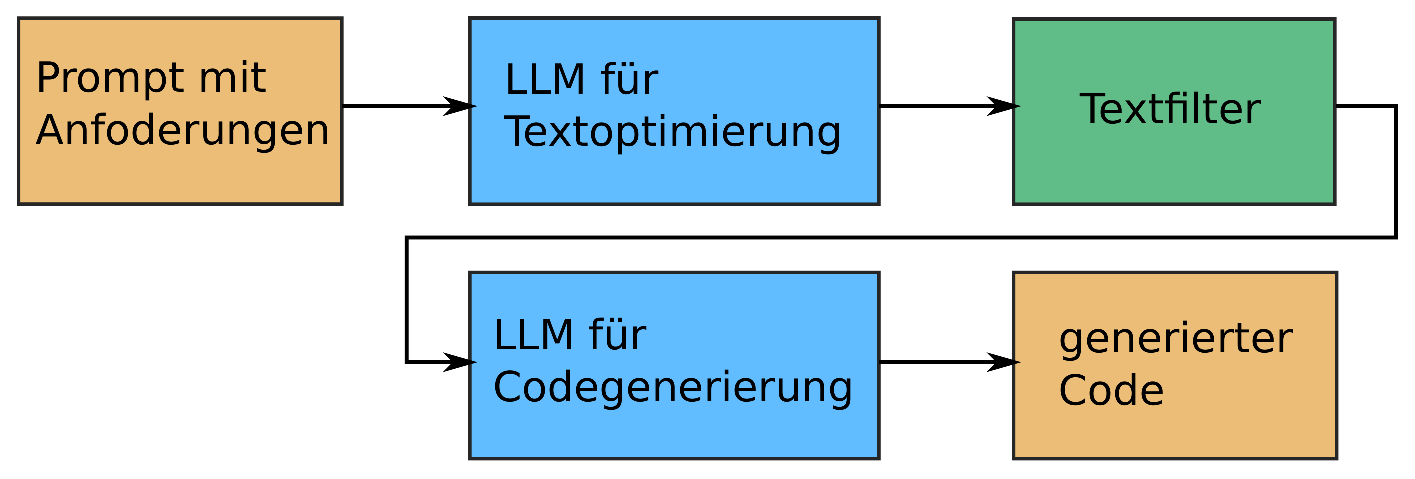
\includegraphics[width=0.8\textwidth]{content/chapter_implementation/images/orchestrierung_llms.eps}
%	\centering
%	\caption{Orchestrierte LLM's für die Codegenerierung}
%	\label{img:orchestration_llms}
%\end{figure}

%\section{Online Modelle}
%Text.

\subsection{Ergebnisse generieren}
Nachdem die Modelle bereitstehen, erfolgt das Generieren der Ergebnisse für jedes einzelne Modell. Mit Prompts, die aus den Proben des HumanEval-XL Benchmark bestehen, werden die Modelle mehrmals hintereinander abgefragt. Die vollständig generierten Antworten der Modelle werden, für eine spätere Auswertung und Nachvollziehbarkeit im \textit{JSONL}-Dateiformat gespeichert. Für jedes Problem erfolgen fünf Abfragen an jedes Modell. Welche Modelle für die Generierung verwendet wurden, ist in Kapitel \ref{subsec:llm_selection} nachzulesen. Alle Modelle wurde von Ollama-Framework bereitgestellt. Das Listing \ref{lst:python_generation_code} zeigt eine einfache Eingabeaufforderung, die an ein Modell gesandt wird.\vspace{0.2cm}

\begin{lstlisting}[
	language=Python,
	caption={Interaktion in Python mit Ollamaserver},
	label=lst:python_generation_code
]
from langchain_ollama.llms import OllamaLLM
from langchain.prompts import PromptTemplate

sample = read_sample_by(task_id=task_id)

model: OllamaLLM
answers: list = []
template = PromptTemplate(
    input_variables=["prompt"],
    template="{prompt}"
)
prompt = template.invoke({"user_prompt": sample.get("prompt")})

for index in range(0, 5):
    answers.append(model.invoke(prompt))

write_result(sample=sample.get("task_id"), answers=answers)
\end{lstlisting}

Nachdem die Proben in Zeile vier vom HumanEval-XL Benchmark eingelesen sind, wird in Zeile sechs bis zwölf das Modell und das Prompttemplate initialisiert. Um die Information \texttt{sample.get("prompt")} aus den Proben zu lesen, wird hier auf den Aufbau der Proben hingewiesen der in Kapitel \ref{subsec:structor_of_humaneval_xl} beschrieben wurde. Anschließend wird das Modell fünfmal abgefragt, hieraus lassen sich später, nach der \texttt{pass@k}-Methode, mit \texttt{k=\{0,...,5\}}, die Modelle evaluieren. Zum Schluss werden die Ergebnisse wie in Zeile siebzehn gezeigt, in JSONL-Dateien abgespeichert.

%---------------------------------------------------------------------------------------------------


\section{Optimierung der Antworten durch Änderung des Frameworks}
Wie das \texttt{langchain} Framework basiert das \texttt{DSPy} ebenfalls auf Python und eignet sich für die Abfrage lokale Ollama Modelle. Somit kann der vorhandene Ollama-Server genutzt werden.
Das Listing \ref{lst:python_generation_code_with_dspy} zeigt die einfache Initialisierung einer Interaktion mit einem lokalen Ollama Models mithilfe der \texttt{DSPy} Bibliothek.\vspace{0.2cm}

\begin{lstlisting}[
	language=Python,
	caption={Interaktion in Python mit Ollamaserver},
	label=lst:python_generation_code_with_dspy
]
import dspy

class BasicProgramming(dspy.Signature):
    question = dspy.InputField(desc="Eine Frage zu PHP Programmierung")
    answer = dspy.OutputField(desc="Generiere Programmcode")

model: dspy.LM = dspy.LM(
    api_base="http://192.168.1.56:11434", # required
    model="ollama_chat/deepseek-r1:32b", # required
    api_key="", # required
    temperature=0.2, # optinal
    cache=False, # optinal
    cache_in_memory=False, # optinal
)

dspy.configure(lm=model)
model(messages=[
    {
        "role": "user",
        "content": "Du bist erfahrener PHP Entwickler",
    }
])

chain = dspy.ChainOfThought(BasicProgramming)
\end{lstlisting}

Der Code zeigt Nach dem Bibliotheksimport wird die Signatur für die Abfrage erstellt. Hier wird die Interaktion mit dem Modell definiert. Es wird die erwartete Eingabe (\texttt{question}) und Ausgabe (\texttt{answer}) festgelegt. Die \texttt{desc}-Parameter im \texttt{InputField} und \texttt{OutputField} dienen lediglich für eine Beschreibung der Felder und haben keinen Einfluss auf den generierten Code.\vspace{0.2cm}

Im Anschluss wird das Lokale Modell mit erforderlichen und optionalen Parametern konfiguriert. Die Parameter \texttt{api\_base}, \texttt{model} und \texttt{api\_key} sind erforderlich. Wobei der Wert für \texttt{key} leer bleibt, solang der Ollama-Server keine Keys für die Anmeldung verwendet. Der Zusatz \texttt{ollama\_chat} veranlasst das Modell-Objekt nach einem Ollama-Server unter der, in \texttt{api\_base} angegebenen IP zu suchen. Mit einer \texttt{temperature}-Angabe von \texttt{0.2} wird das Modell zu einer deterministischen Antwort geleitet. Hier ist eine hohe Kreativität nicht gewünscht. Werden die optionalen Parameter \texttt{cache} und \texttt{cache\_in\_memory} nicht gesetzt, so wird ein Cache eingesetzt, was dazu führt, dass die Abfrage nur einmal in die LLM leitet und die Antwort in einem Cache abgelegt wird. Bei allen weiteren Anfragen würde diese Antwort wiederholt zurückliefert. Das würde bedeuten, das immer nur der $pass@k$ für $k=1$ erstellt werden könnte. Um dies zu verhindern, müssen beide Parameter den Wert \texttt{False} erhalten.\vspace{0.2cm}

Nachdem das Modell konfiguriert ist, wird in Zeile 16 DSPy mit dem Modell \texttt{model} konfiguriert und definiert somit deren Verwendung. Ab der Zeile 17 wird dann die Systemnachricht initialisiert. Diese Systemnachricht wird als erste Nachricht an die LLMs gesendet und legt dadurch den Kontext fest.\vspace{0.2cm}

Die letzte Zeile des Listings \ref{lst:python_generation_code_with_dspy} zeigt die Erstellung einer \texttt{ChainOfThought} Instanz mit der zuvor erstellten Signatur.


\subsection{Ergebnisse generieren}
\begin{tcolorbox}[
	enhanced,
	colback=red!5!white,
	colframe=red!75!black!50,
	title= Mein roter Faden
	]
	Mögliche Optimierungsstrategien
	\begin{itemize}
		\item mit dem Model Programming (DSPY) Ansatz: Python Bibliothek vorhanden \href{https://pypi.org/project/dspy/}{pypi.org | DSPy}.
	\end{itemize}
\end{tcolorbox}

%---------------------------------------------------------------------------------------------------


%\subsection{Auswertung der Modellantworten}
\section{Benchmark Codeevaluation}\label{sec:benchmark_evaluation}
Die Analyse der generierten Antworten muss für jedes Modell individuell angepasst werden, da die erzeugten Codefragmente zwischen den Modellen variieren. Insbesondere unterscheiden sich die Formate, in denen die Codesnippets generiert werden, beispielsweise durch \texttt{```php} oder \texttt{```php \textbackslash n <?php}. Dementsprechend erfordert die Extraktion des relevanten Codes aus den Modellantworten eine flexible Methode, die an das jeweilige Ausgabeformat der Modelle angepasst wird. Ein exemplarischer Lösungsansatz zur Extraktion des generierten Codes ist in Listing \ref{lst:code_extraction} dargestellt.\vspace{0.2cm}

\begin{lstlisting}[
	language=Python,
	caption={Codesnippet zur Extrahierung des Codes aus der LLM Antwort},
	label=lst:code_extraction
]
def get_generatet_code(code=code):
    if len(code.split("```php")) > 1: # find start
        code = code.split("```php")[1]
        code = code.split("```")[0]

    if code.startswith("<?php"): # find start
        code = code.split("<?php")[1]
        code = code.split("?>")[0]

    if len(code.split(r"\n}\n")) > 0: # find end
        code = code.split(r"\n}\n")[0] + "\n}\n"

    return code
\end{lstlisting}

Um den generierten Code zu evaluieren, wird dieser zusammen mit dem Test, der jeweiligen Probe aus dem Benchmark zusammengeführt. Das Ergebnis ist ein ausführbarer Code, der die geforderte Methode enthält. Mittels Python wird der Code getestet, ob der dieser ausführbar ist. Entsteht bei der Ausführung ein Laufzeitfehler erfolgt der Abbruch des Tests. Dieser kann ausgelöst werden durch eine nicht korrekte Syntax, einer Endlosschleife oder wenn die geforderte Methode nicht generiert wurde. All diese Ereignisse führen dazu, das die Probe als nicht bestanden gilt. Das Listing \ref{lst:php_interpreter_in_python} zeigt den Ausschnitt im Code zur Ausführung des PHP Interpreters in Python.\vspace{0.2cm}

\begin{lstlisting}[
language=Python,
caption={Codesnippet zur Ausführung des PHP Interpreters},
label=lst:php_interpreter_in_python
]
import subprocess

def test_answer(task_id, repetition):
    # read generated code
    answer = read_answer(task_id=task_id, repetition=repetition)
    answer = get_generatet_code(code=answer)

    # read test in HumanEval-XL
    test = read_sample(task_id=task_id).get("test")

    try:
        result = subprocess.run(
            ["php", "-r", f"{test}{answer}"],
            capture_output=True,
            text=True,
            check=False,
            timeout=5,
        )
    except subprocess.TimeoutExpired:
        return False

    if result.stderr.strip() == "":
        return True

    return False
\end{lstlisting}

Nachdem eine von fünf Antworten des Modells und der Test aus dem Benchmark vorliegen, erfolgt die Prüfung des generierten Codes. Diese wird im Listing \ref{lst:php_interpreter_in_python} ab Zeile zwölf gezeigt. Die Funktion liefert \texttt{True} zurück, wenn es keine Fehler im Test gab, sonst immer \texttt{False}. Das Exception-Handling ab Zeile 19 wird aufgerufen, wenn die PHP Ausführung in einer Schleife hängt. Hier wird ein \texttt{Timeout} abgefangen und somit gibt der Test als nicht bestanden. Aus den erhaltenen Ergebnissen, der Proben eines Tasks, berechnet die \texttt{pass@k} Methode, die \glqq Wahrscheinlichkeit das in \texttt{k}-Proben, eine korrekte Probe ist\grqq \, hinsichtlich Codegenerierung. Anschließend wird der Durchschnitt für die Zuverlässigkeit des Modells errechnet.\vspace{0.2cm}

\textbf{Umsetzung der pass@k Metric}\vspace{0.2cm}

Nach Abschluss der Tests werden die Ergebnisse mithilfe der \textit{pass@k}-Methode analysiert. In Python steht hierfür, die Bibliothek \textit{pass\_at\_k} zur Verfügung. Das Listing \ref{lst:custom_pass_at_k} zeigt die Implementierung der Methode gemäß Gleichung \ref{equ:pass_qt_k_complex} in Kapitel \ref{subsec:pass_at_k}, wie sie auch in der Python-Bibliothek verwendet wird.  


\begin{lstlisting}[
	language=Python,
	label=lst:custom_pass_at_k,
	caption={Berechnung der pass@k Metrik in Python}
]
def custom_pass_at_k(n: int, c: int, k: int) -> float:
    """
    :param n (int): numbers of total samples.
    :param c (int): number of currect samples.
    :param k (int): number of consider samples.
    """
    if n - c < k:
        return 1.0
    return 1.0 - np.prod(1.0 - k / np.arange(n - c + 1, n + 1))
\end{lstlisting}

%Die \textit{pass@k}-Methode dient zur Berechnung der Wahrscheinlichkeit, dass in $k$ Abfragen mindestens eine korrekte Lösung enthalten ist. Dazu
Die Methode erwartet drei Parameter. Der Parameter $n$ bezeichnet die Gesamtanzahl der Abfragen pro Probe. Der Parameter $c$ gibt die Anzahl der korrekten Abfragen innerhalb einer Probe an. Schließlich legt der Parameter $k$ fest, wie viele der besten Abfragen für die Bewertung berücksichtigt werden. Alle drei Parameter sind ganzzahlig (\texttt{Integer}), während das Ergebnis als Gleitkommazahl (\texttt{Float}) zurückgegeben wird.  

In dieser Arbeit werden die Werte $k=1$ und $k=5$ für die Evaluierung herangezogen. Nachdem jede Probe des HumanEval-XL-Benchmarks einzeln bewertet wurde, wird eine aggregierte Bewertung für das gesamte Modell ermittelt. Diese Berechnung erfolgt gemäß Gleichung \ref{equ:probability_of_success_per_model} in Kapitel \ref{subsec:pass_at_k}.  

% --- More Tests -----------------------------------------------------------------------------------


%\section{Codeevaluation mit Frameworks}
%Neben der bekannten Evaluationsmethode mit dem HumanEval Benchmark, wird hier eine weitere Testmethodik überprüft, die mit verschiedenen Validierungstools der jeweiligen Programmiersprache ausgeführt wird. Für die Erstellung der Abfragen wird das Python-Skript verwendet, was schon im Kapitel \ref{sec:benchmark_evaluation} vorgestellt wurde.

%\subsection{PHP Codeevaluation}
%Der Test wird bei den erweiterten Problemen durchgeführt und beginnt mit den Unit-Tests die mit \textit{PHPUnit} durchgeführt werden. Im Anschluss wird \textit{PHPMetrics} ausgeführt. Hierbei wird geprüft, ob die Codekomplexität und Wartbarkeit überprüft. Die Ausführung der Tests wird mithilfe eines Python-Skripts durchgeführt. Es wird eine PHP Datei erstellt, die mit den Frameworks geprüft wird.

%\subsection{JavaScript Codeevaluation}
%Text.

%\section{Online Modelle}
% Eigenen KI Server \href{https://www.computerweekly.com/de/ratgeber/Einen-KI-Server-mit-Ollama-und-Open-WebUI-einrichte}{Computer Weekly}
% Orchestrierung mit Python \href{https://pypi.org/project/multillm/}{multillm-Projekt}
% LangChain Library \href{https://python.langchain.com/api_reference/ollama/chat_models/langchain_ollama.chat_models.ChatOllama.html}{Example}
% \href{https://pypi.org/project/langchain-ollama/}{Python lib langchain-ollama}
% YouTube \href{https://www.youtube.com/@AICodeKing}{AICodeKing}